%%% DOCUMENT BEGIN

\documentclass{IEEEtran}

\usepackage[utf8]{inputenc}

\usepackage{geometry}
\geometry{a4paper}

\usepackage{graphicx}

\usepackage{cite}
\usepackage{amsmath,amssymb,amsfonts}

\usepackage{graphicx}
\usepackage{textcomp}

%%% PACKAGES
%\usepackage{booktabs} % for much better looking tables
%\usepackage{array} % for better arrays (eg matrices) in maths
%\usepackage{paralist} % very flexible & customisable lists (eg. enumerate/itemize, etc.)
%\usepackage{verbatim} % adds environment for commenting out blocks of text & for better verbatim
%\usepackage{subfig} % make it possible to include more than one captioned figure/table in a single float
\usepackage[english]{babel}
\usepackage{mathtools}

%%% HEADERS & FOOTERS
\usepackage{fancyhdr} % This should be set AFTER setting up the page geometry
\pagestyle{fancy} % options: empty , plain , fancy
\renewcommand{\headrulewidth}{0pt} % customise the layout...
\lhead{}\chead{}\rhead{}
\lfoot{}\cfoot{\thepage}\rfoot{}

%%% SECTION TITLE APPEARANCE
%\usepackage{sectsty}
%\allsectionsfont{\sffamily\mdseries\upshape}

%%% ToC (table of contents) APPEARANCE
%\usepackage[nottoc,notlof,notlot]{tocbibind} % Put the bibliography in the ToC
%\usepackage[titles,subfigure]{tocloft} % Alter the style of the Table of Contents
%\renewcommand{\cftsecfont}{\rmfamily\mdseries\upshape}
%\renewcommand{\cftsecpagefont}{\rmfamily\mdseries\upshape} % No bold!


%%% END Article customizations

\renewcommand{\baselinestretch}{1.2} 
%%%%%%%%%%%%%%%%%%%%%%%%%
%%%          Fill in the title details                      %%%

\def \thetitle {INF-3701 - Advanced Database Systems}
\def \thesubtitle {Assignment 2}
\def \theauthor {Thomas B Nilsen and Valter Berg}
\def \pagecount {6}

%%%%%%%%%%%%%%%%%%%%%%%%%

%\pagestyle{fancy}
\pagestyle{fancyplain} % options: empty , plain , fancy
\renewcommand{\headrulewidth}{1pt} % customise the layout...
\renewcommand{\footrulewidth}{0pt}
\lfoot{}\cfoot{Page {\thepage} of \pagecount}\rfoot{}

\begin{document}

\title{Data Mining in Medical Data}

\author{\IEEEauthorblockN{Valter Berg}
\and
\IEEEauthorblockN{Thomas Bye Nilsen }
}
\maketitle
%%% TABLE OF CONTENTS

%\tableofcontents


%\newpage{}

%%% DOCUMENT BODY

%%% Set counter to 1
\setcounter{page}{1}

\section{Abstract}

We observe an ever-increasing quantity of data being produced in medical areas. The data originates from different sources throughout the research field. The diversity of the data and its properties make it challenging to process the data within a reasonable amount of time. To meet the demand for useful results distilled from large collections of data, new techniques are called for. To analyze big data, various data mining algorithms have been applied which extract useful pieces of information that are hidden a large datasets. In this paper we review some of the applied techniques, look for any shortcomings and give suggestions for the remaining challenges. How will the suggested designs fit as theoretical solutions?

\section{Introduction}
There is a vast and rapidly expanding amount of data being produced digitally. In the US healthcare system alone, in 2011, 150 exabytes of data was stored. Continuing at this rate of growth, as stated in a report, the size of the volume will reach the zettabyte scale, and not long after that, the yottabyte scale \cite{intro}. When the physical properties of the data increases beyond a critical point, new techniques, architecture, algorithms and visualization of the data are required to use the data in a meaningful context. This has caused a rapid development in computer science research to gain insights into large collections of data, or big data, that have not been achieved earlier. This rapid development has mainly been unfolding within the disciplines like internet business and finance, while in the healthcare area, the progress has not been as widespread. However, there seems to be an increasing attention to big data in the healthcare sector. A survey is predicting that the outcome will be severely beneficial for the sector.\cite{gg}


\subsection{Medical big data}
Medical big data consists of large quantities of diverse medical data. The data originates from hospitals, pharmaceutical companies and academic environments. The datasets can be categorized based on their origin. Some of the categories are administrative claim records, clinical registers, electronic health records, biometric data and large clinical trials. The value of the data lies in the processing and interpretation of the datasets. The datasets in the different categories, which are likely to be heterogeneous in terms of format and completeness, can be linked together as well. It can be valuable to link heterogeneous datasets together to search for related data that is otherwise inaccessible.\cite{wp}
\\\\
An example where integration of heterogeneous datasets is needed is when it is possible gain insight into the relation between patients' conditions and environmental events. A 360-degree view of a patients integrated with environmental data or even medical metrics yields insight into the relation between the two datasets. Facts regarding epedemic trends described in natural language text can be linked to a database containing patterns that match the trend. \cite{integration}
\\\\
Medical big data can also be hard to access due the lack of data-sharing intensives and in some cases, the lack of guarantees that untrusted third-parties will not be able to access the data. This is a serious privacy concern. 
\\\\
For patient records, there might be valuable information regarding previous treatments, given parameters like geographical region, age, gender and other biological properties. Relatively large datasets from hospitals across the industry, both public and private, possess such collections. Insights into these datasets could yield information regarding past and present patient treatment, use of medical resources and suggestions to future treatments. By grouping together patients, one could profile patients and review the treatment strategies. Because it is not possible to conduct enough trials to cover all types of patients, it could be crucial that enough evidence is gathered. \cite{mbd3}
\\\\
Administrative claim records explain how healthcare resources are utilized and the outcomes of such use. Overview of economic status of an institution is important to administer resource usage. By looking at the records, one can see how different research projects and medical treatment projects are funded. Then, it is possible to balance the funding with respect to the funding resources available. 
\\\\
Clinical registers is closely related to patient records.\cite{geir} They contain information regarding the health status of patients and the treatments they receive over varying periods of time. They typically focus on the common reason for needing health care and how patients with various characteristics respond to various treatment methods. 
The clinical records can be compared to find patterns between patients with various characteristics that might prove to be helpful in finding new methods for treatments.



\subsection{Motivation}
There are several reasons for using new techniques in medical big data processing. There are several challenges the industry faces that the current technology is not able to overcome. First of all, there are missing values in the case of electronic patient records\cite{wp}. When records or attributes within records are missing, their absence yields an incomplete picture and low value of the dataset. This issue is traceable throughout even large datasets, which in turn can concern the industry to a relatively large degree. 
\\\\
In the case of curse of dimensionality has also proven to be a problem.
This is the case of an excessive number of dimensions in the datasets. As the number of dimensions increases, the complexity for processing the datasets and the volume for storing the data increases rapidly as well. 
\\\\
Data standardization is also a challenge. The format in which the data is stored and processed can vary across institutions and companies . On a large scale across the industry, even across country borders, the standards can vary to a relatively large degree. The difference in formats can, in turn, prove to be challenging when related datasets are to be processed. Data mining of different datasets will therefore require different algorithms which can be time-consuming for researchers. 
\\\\
To some degree related to the lack of data standardizations, about 50\% of all data in medical datasets are considered to be unstructured\cite{wp}. The unstructured data mainly consist of free-text reports and is used in communication between healthcare providers. The free-text can be from nurse notes, blood tests, or physiological data and it has no standard template on its appearance. This heterogeneity in free-text data has to be considered when extracting information from it with data mining techniques. Although there have been more research applied to the field of data mining in medical health data, there is still room for more development, as depicted in this paper. Increased funding in medical big data will improve medical treatments and benefit patients for generations to come. 


\section{Techniques}
For some issues listed above, there exist solutions that partly overcome the challenges. For missing values, it is proposed to omit the data point. However, this may lead to loss in information and tampering of integrity. However, this method is overused in a practical context. \cite{wp} A suggestion is to use different techniques used in statistics. One technique is to estimate variance and covariance derived from maximum likelihood methods. This method is based on observing previous events. Previous events might involve other patients' records. The other algorithm is listwise detection. These two methods are used in datasets that suffer from MAR (missing at random) values. \cite{statistics} The patients' privacy concern becomes relevant at this point. There must be no connection between two patients' identity, nor it can be possible to backtrack the calculation that points to a particular patient. 
\\\\
Another technique is imputation. Imputation is based on estimating substitute values based on other, for example from other similar datasets. \cite{imputation}. The datasets can be patients with similarities. 
\\\\
Several techniques have been proposed to solve curse of dimensionality. \cite{cod} lists several methods to that can be used. One is DQC which has the ability to expose hidden structures and determine their significance in high-dimensional big data. It outlines correlated variables in the higher dimensions. One can look at it as a summery of the higher-dimensions. Another is feature hashing (FH). It is based on hashing the ID of the higher-dimensional feature. In this way, it is possible to reduce the storage space in the lower dimensions. 
\\\\
The issue regarding data standardization can be solved by agreeing on a standardized format that is traceable throughout the industry and research area. \cite{who} established a forum consisting of over 200 individuals from 54 countries contributed to the dialogue on standardization and interoperability. In other words, there have been willingness to achieve this goal, yet there seems to be vastly more work to do.  Representatives from institutions and companies must come together and agree on a set of formats compatible with existing technology and algorithms, which also retains patients’ privacy rights. The challenge of standardizing is amplified by the presence of unstructured data. A potential solution can be applied to the input and output of the data mining algorithm. At the input side, a format can be determined so that a larger percent of the input data is structured. At the output end, the data can also be formatted in a determined format adhering to some standard.
\\\\
Regarding the challenges with extracting information from free-text in medical data the research group Jensen, K. et al.\cite{freetext} worked on identifying cancer patient trajectories with analysing free text in electronic health records. Their goal was to identify cancer patient trajectories in need of resource demanding treatment and repeated hospital admissions. They concluded that their tool for identifying patient trajectories through free text analyses would be sufficient to use as a data-driven support tool in the complete cancer trajectory. They also claimed that use of their tool could decrease adverse events and readmissions and improve the quality of cancer care. 
TODO: DESCRIBE FIGURE 1 HERE SOMEWHERE. 

\begin{figure}[]
\begin{center}
\fbox{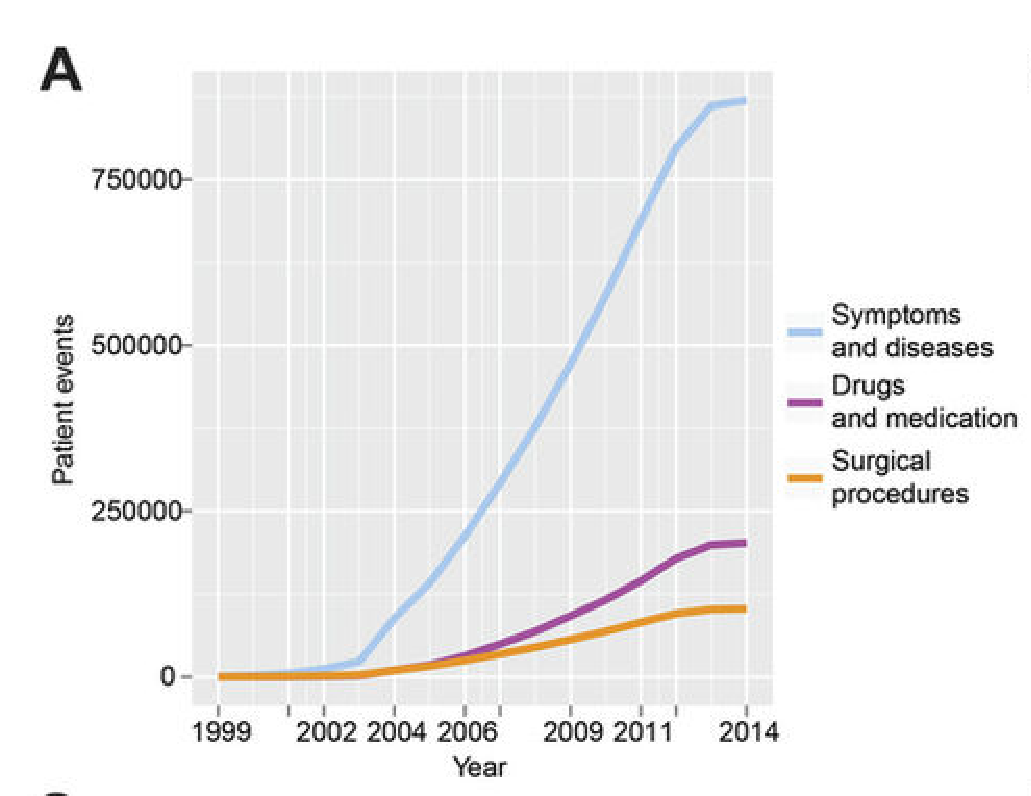
\includegraphics[width=210px]
{patientEvents.pdf}}
\end{center}
\caption{Patient events in terms of symptoms and diseases (blue), drugs, medication (magenta) and surgical procedures (orange) accumulated over time in the EHRs at UNN.\cite{freetext}}\label{fig:ackseq}
\end{figure}
 

Here is a nice technique discussed.\cite{medicalmining}

\section{Discussion}
As we have seen, there are still some challenges that need to be addressed. Overcoming the challenges needs to be prioritized by governments across country borders. Despite the fact that the suggestions are theoretical, they are supported by reasoning. In the years to come, as the population and medical research grow in size, investments must be done. We have covered a subset of the challenges there is; there are more to shortly mention. One is regulatory compliance issues\cite{kek} which involves legal challenges that can surface in the process of storing and processing large amounts of data. Data storing and processing must comply according to government regulations, as is the case for CancerLinQ \cite{gouvernment}.
\\\\
Lack of appropriate skills can act as a barrier in implementing big data systems\cite{kek}. With change in technology, techniques and treatment standards, the personnel operating the systems must have up-to-date knowledge and skills.
Even though there have been decades of research, there is still a risk of adverse events and mortality in cancer treatment today. With continuously assessing patient related risk factors the treatment can be optimized, adverse events avoided and number of hospital readmissions decreased. As mentioned the research  from Jensen, K. et al. adapted to this concern with assessing patient related risk factors. As their results revealed, they achieved a mechanism that can be used as a tool when conducting patient trajectories. This is a valid example on how the data stored in EHR in the healthcare sector can be utilized to improve the medical treatment structure. 

 
\section{Conclusion}
Although there have been more research applied to the field of data mining in medical health data, there is still room for more development, as depicted in this paper. Increased funding in medical big data will improve medical treatments and benefit patients for generations to come. As we have seen, there is room for improvements. As in any other area, there will only become more data to store and process. Addressing the challenges is the first step towards implementing solutions. Several papers, on which this paper is based, have addressed these challenges. It shows that there is willpower to solve the remaining issues. 


%%% BIBLOGRAPHY

%\newpage{}


\bibliographystyle{plain}
\bibliography{report}



\end{document}
